\section{Experimentos e Resultados}

Para comparar o desempenho entre o PostgreSQL e o Citus, executamos os benchmarks TPC-C em ambos os sistemas.
No caso do citus, utilizamos uma configuração de 3 nós trabalhadores e 1 nó coordenador. Além disso, para simular um ambiente de cloud, cada instância foi limitada a 8GB de RAM e 2 CPUs,
além da introdução de latência de rede aleatória (150us $\pm$ 200us). 

A carga e o benchmark foram executados durante um período 5 minutos, 
com o número de usuários igual a 64 usuários, e parâmetro do benchmark warehouses = 40.

Os resultados foram coletados e analisados utilizando o Grafana e o Prometheus,
e serão discutidos nas seções a seguir.

Vale ressaltar que no caso dos gráficos do Citus, os resultados foram coletados do nó coordenador,
que é o responsável por coordenar as consultas e distribuir as tarefas entre os nós trabalhadores. 

Os gráficos a seguir mostram o desempenho do sistema durante a execução do benchmark:
\subsection{Resultados do TPC-C}
\begin{figure}[H]
	\centering
	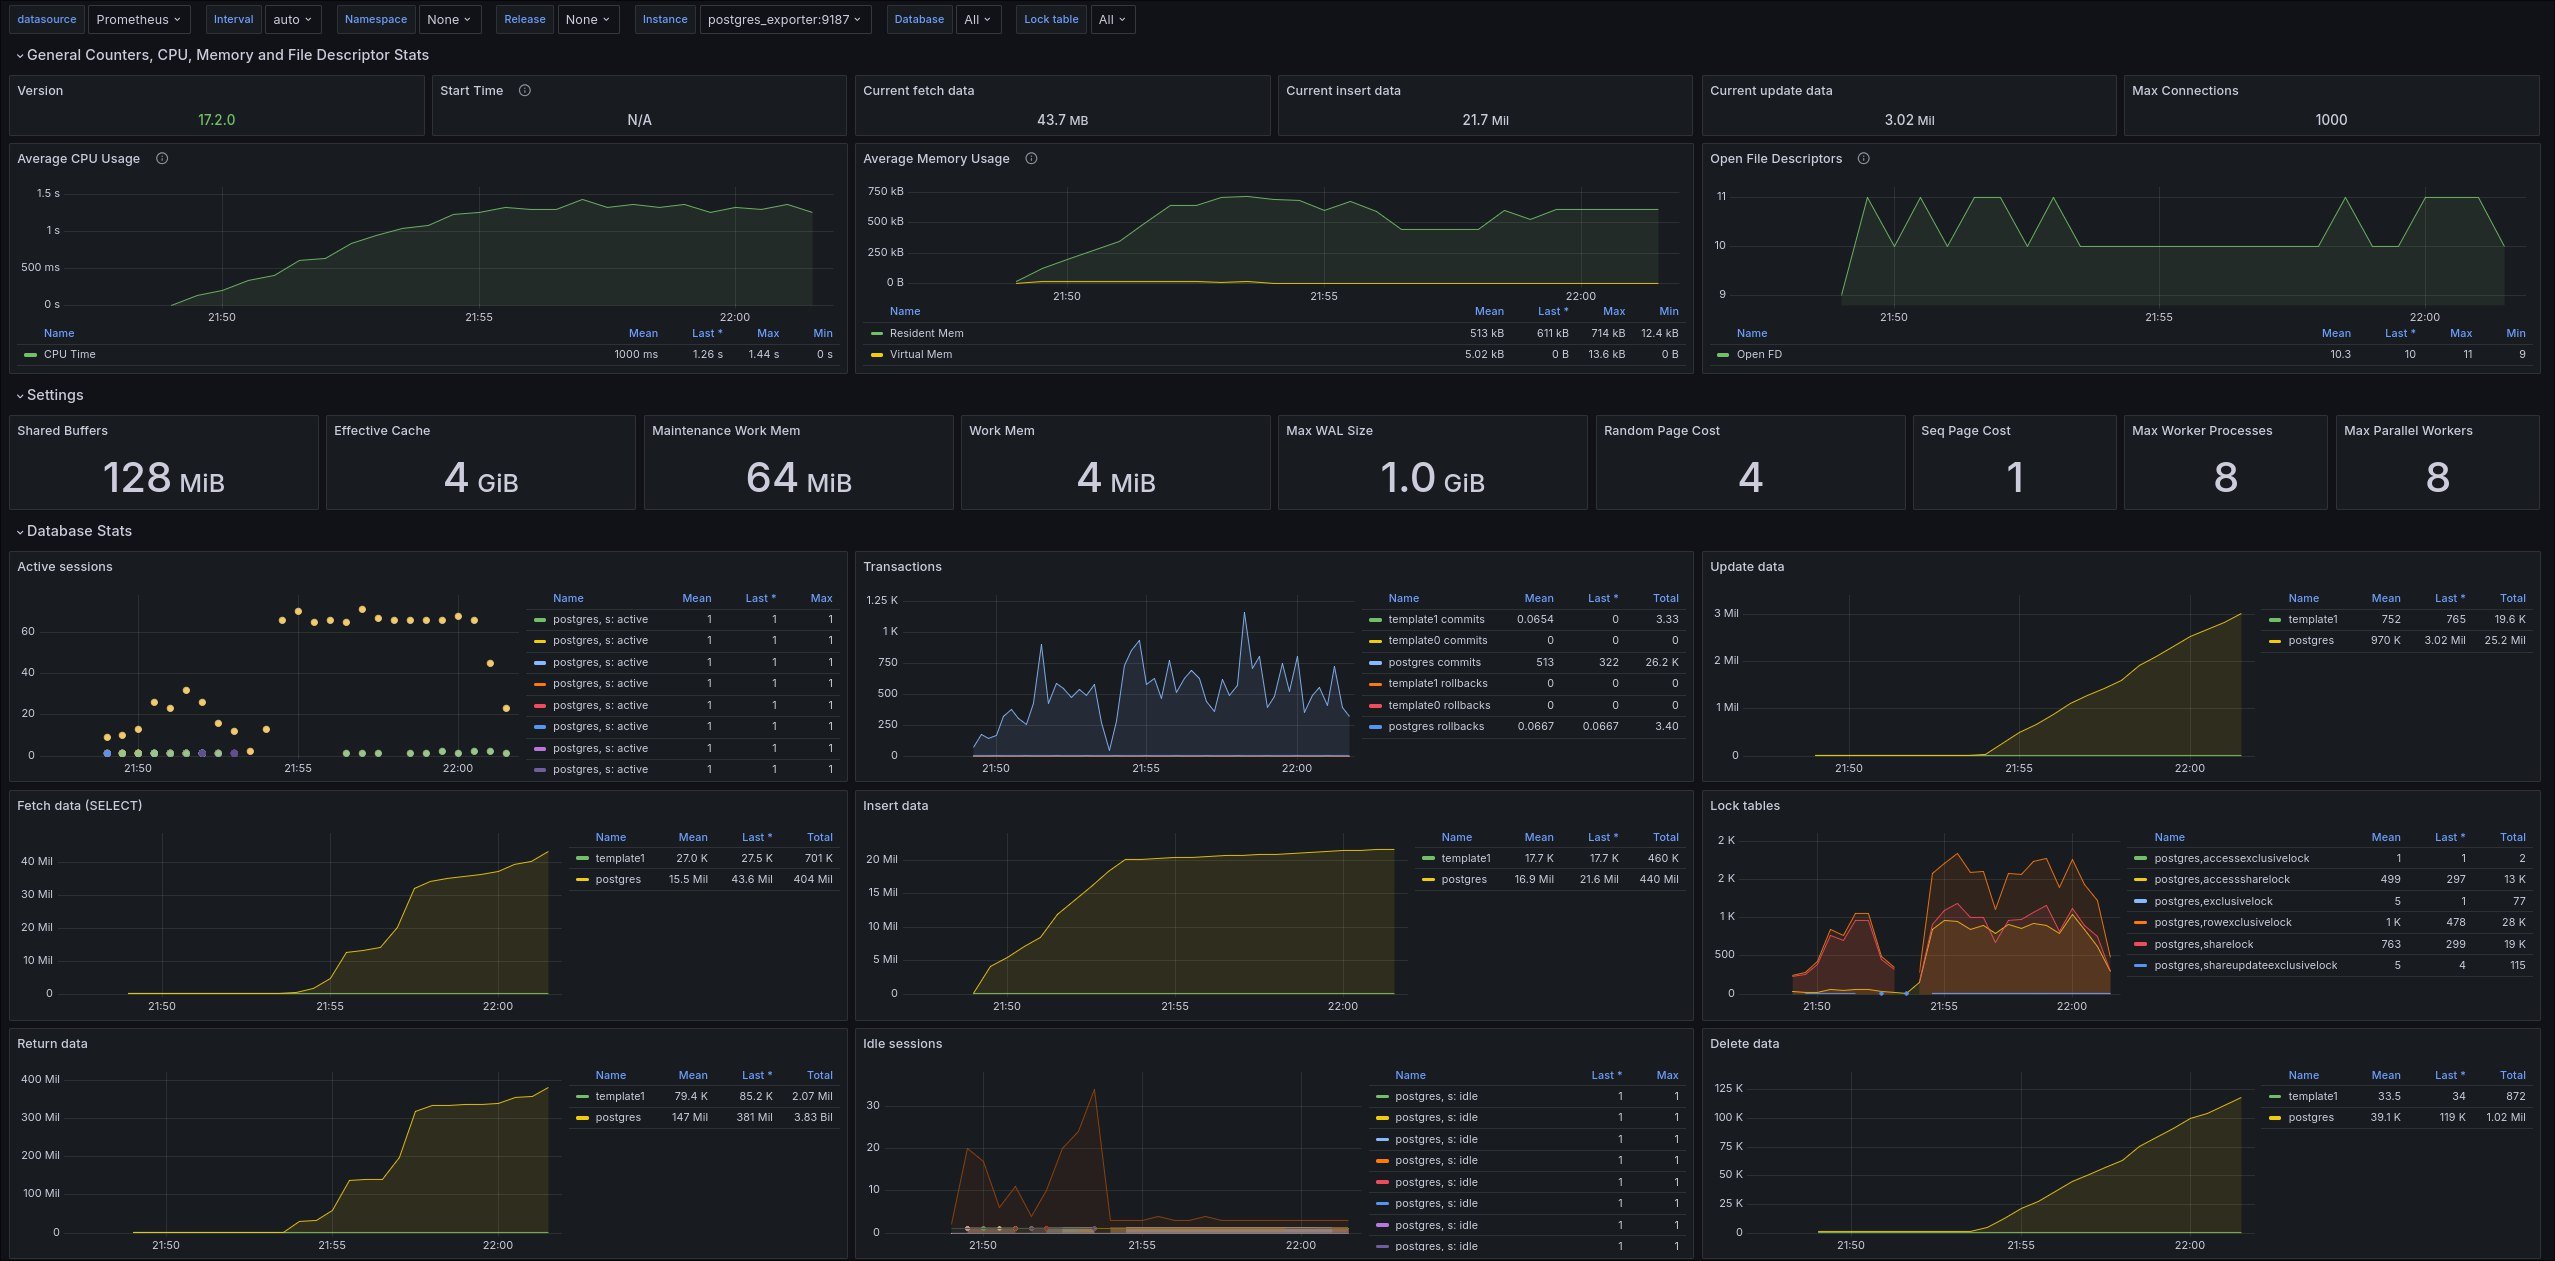
\includegraphics[width=0.8\textwidth]{imgs/citus.jpg}
	\caption{Resultados do TPC-C para o Citus}
	\label{fig:tpc-c}
\end{figure}

\begin{figure}[H]
	\centering
	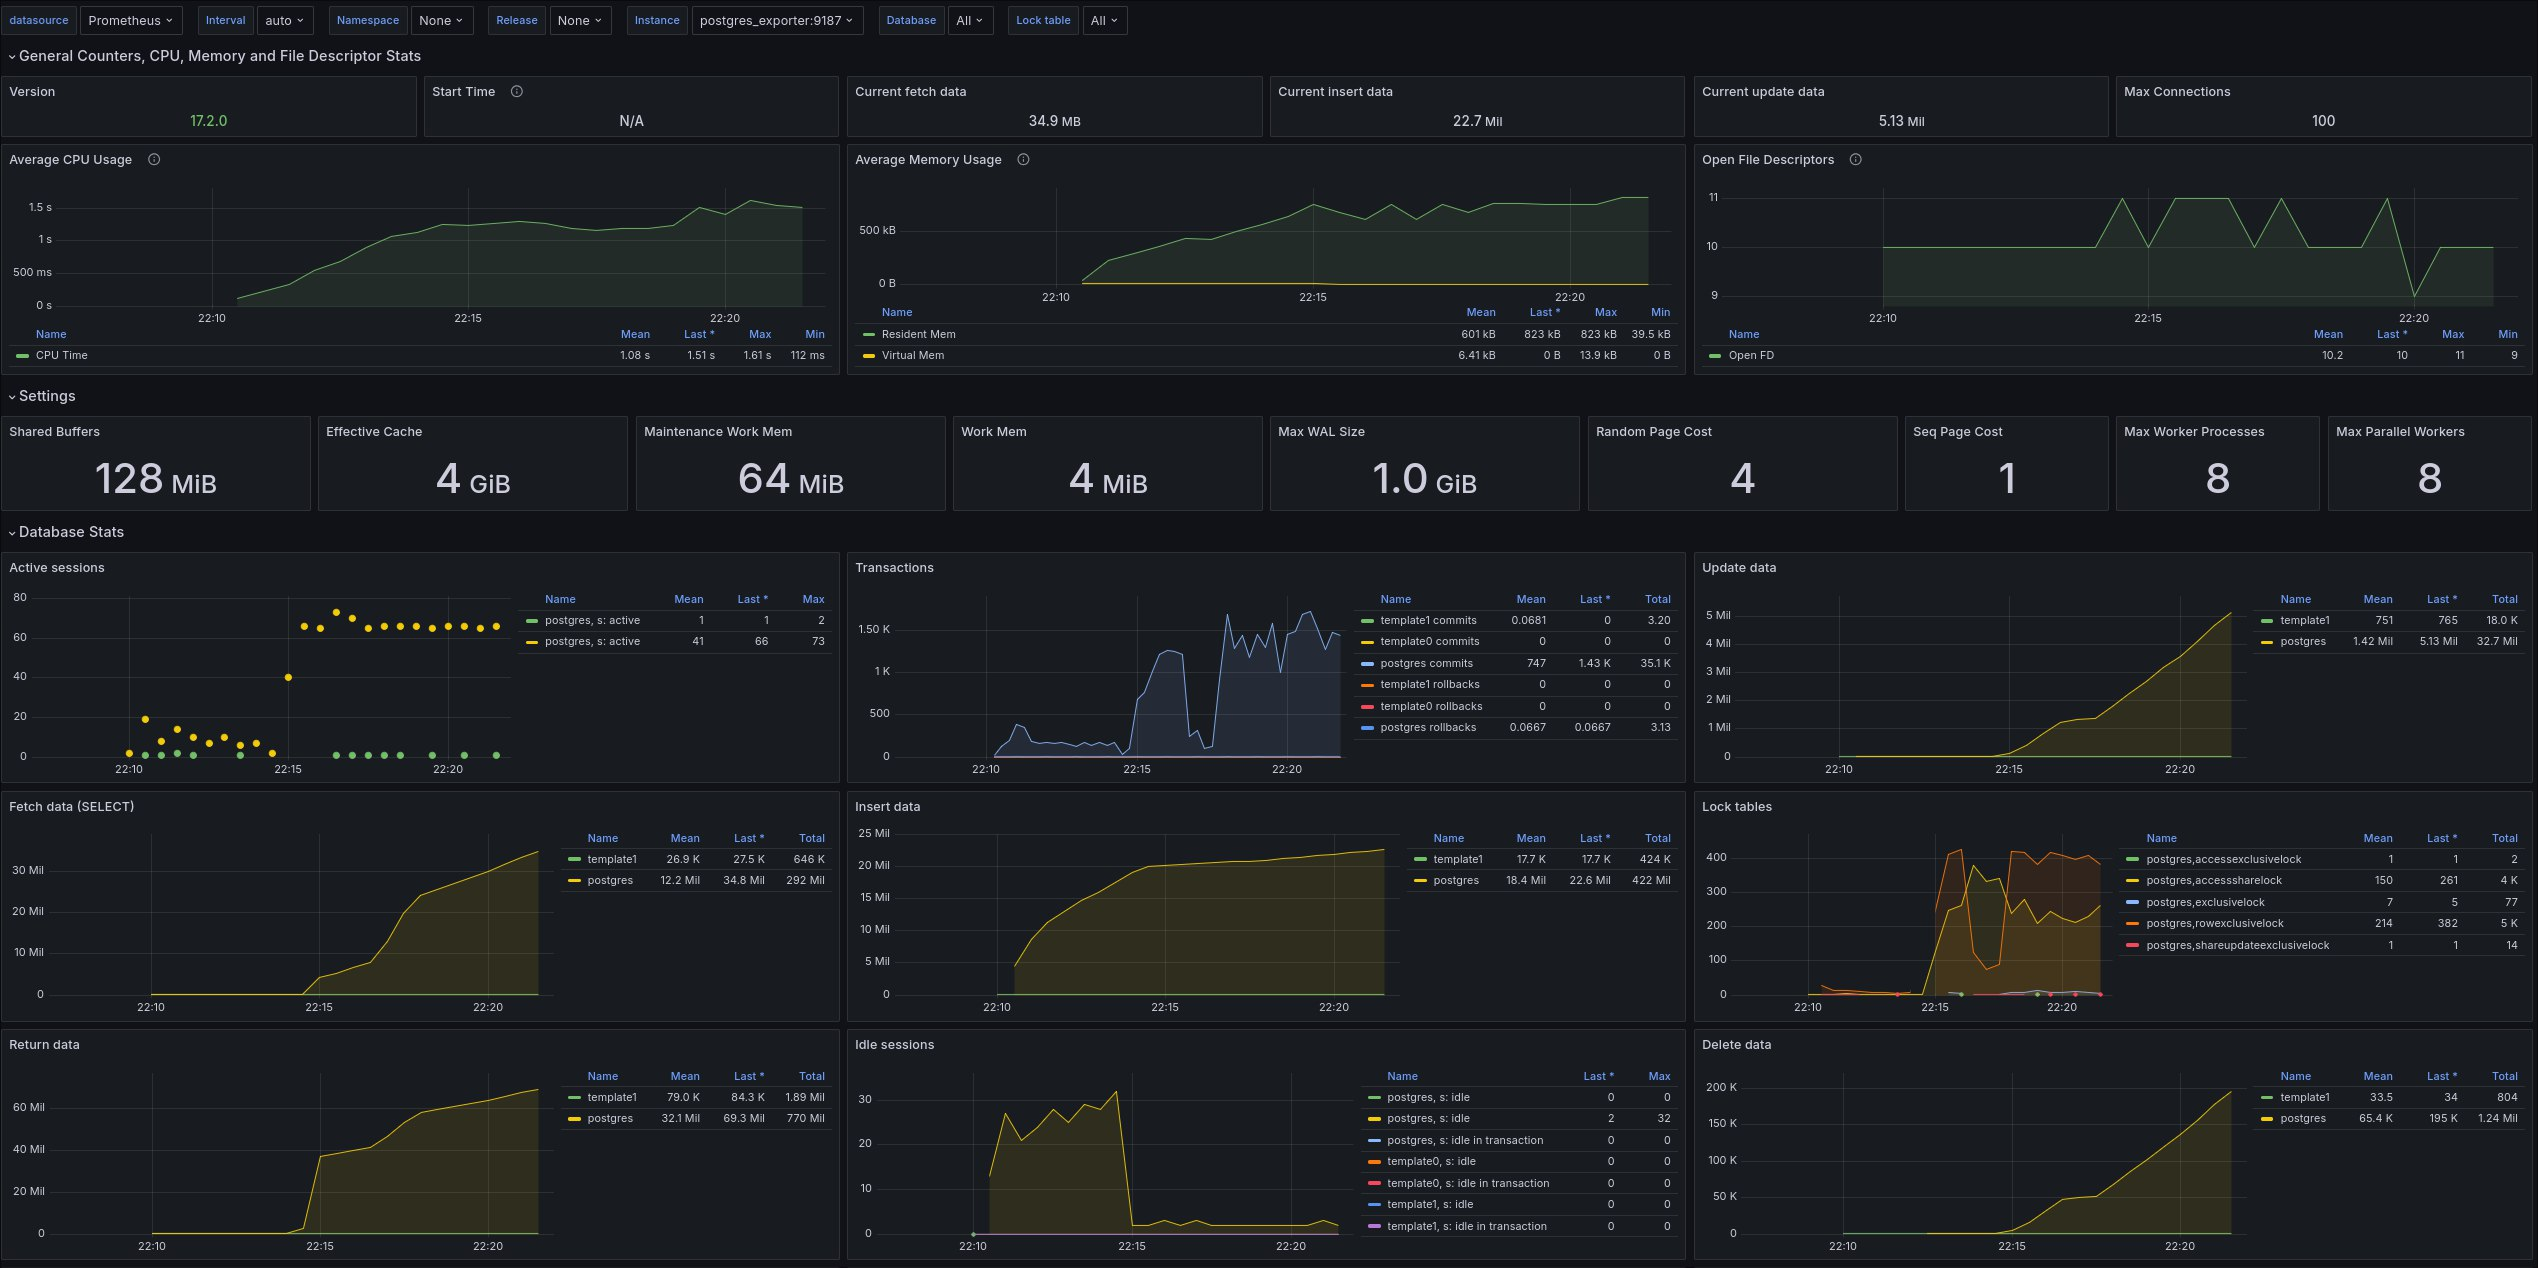
\includegraphics[width=0.8\textwidth]{imgs/Postgres.jpg}
	\caption{Resultados do TPC-C para o PostgreSQL}
	\label{fig:tpc-c}
\end{figure}

Como resultados, obtemos que O PostgreSQL atingiu 31405 operações novas por minuto e 72424 transações por minuto, 
enquanto o Citus atingiu 15304 operações novas por minuto e 35762 transações por minuto.
Além disso, o tempo médio registrado pelas operações do Citus foi o seguinte:

\[
\begin{array}{|l|l|r|r|r|r|}
\hline
\textbf{PROC} & \textbf{Banco} & \textbf{MIN (ms)} & \textbf{AVG (ms)} & \textbf{MAX (ms)} & \textbf{TOTAL (ms)} \\
\hline
PAYMENT & Postgres & \textbf{0.833} & \textbf{52.601} & \textbf{1257.365} & \textbf{34106475.135} \\
        & Citus    & 0.990          & 101.086         & 1767.711          & 36185664.966         \\
\hline
NEWORD  & Postgres & \textbf{1.640} & \textbf{48.569} & \textbf{1255.893} & \textbf{31475935.439} \\
        & Citus    & 1.774          & 107.871         & 1737.546          & 38724729.750         \\
\hline
SLEV    & Postgres & \textbf{0.440} & 153.889         & 21302.445         & 10003419.917         \\
        & Citus    & 0.612          & \textbf{63.438} & \textbf{5600.833} & \textbf{2288143.726} \\
\hline
DELIVERY& Postgres & \textbf{1.278} & \textbf{54.623} & \textbf{1417.772} & 3534810.624          \\
        & Citus    & 2.286          & 115.989         & 1505.085          & \textbf{4142561.285} \\
\hline
OSTAT   & Postgres & \textbf{0.104} & \textbf{2.725}  & \textbf{455.587}  & \textbf{173186.360}  \\
        & Citus    & 0.269          & 7.474           & 609.841           & 262082.364           \\
\hline
\end{array}
\]

\[
\begin{array}{|l|l|r|r|r|}
\hline
\textbf{PROC} & \textbf{Banco} & \textbf{P99 (ms)} & \textbf{P95 (ms)} & \textbf{P50 (ms)} \\
\hline
PAYMENT & Postgres & \textbf{413.035} & \textbf{167.278} & \textbf{27.633} \\
        & Citus    & 611.674          & 352.694          & 72.123 \\
\hline
NEWORD  & Postgres & \textbf{413.374} & \textbf{160.868} & \textbf{23.915} \\
        & Citus    & 607.420          & 362.191          & 83.081 \\
\hline
SLEV    & Postgres & 4235.829         & \textbf{73.669}  & \textbf{6.215} \\
        & Citus    & \textbf{730.162} & 224.685          & 8.710 \\
\hline
DELIVERY& Postgres & \textbf{441.496} & \textbf{191.119} & \textbf{25.470} \\
        & Citus    & 596.206          & 375.478          & 90.453 \\
\hline
OSTAT   & Postgres & \textbf{47.199}  & \textbf{3.844}   & \textbf{1.292} \\
        & Citus    & 80.547           & 60.180           & 2.439 \\
\hline
\end{array}
\]

Nesse contexto, os resultados apresentados evidenciam o overhead do Citus, especialmente em cenários de alta concorrência simulados pelo benchmark TPC-C.

O PostgreSQL standalone alcançou 31.405 operações novas por minuto e 72.424 transações por minuto, 
enquanto o clusterizado atingiu 15.304 operações novas por minuto e 35.762 transações por minuto.
Isso indica que o PostgreSQL foi capaz de processar aproximadamente o dobro de operações e transações por minuto em relação ao Citus,
evidenciando que, nesse cenário, o overhead do Citus superou os benefícios da distribuição de dados e consultas.
Além disso, o tempo médio registrado pelas operações do Citus foi significativamente maior em comparação ao PostgreSQL.

Considerando que ambos os testes foram realizados em um ambiente conteinerizado, é possível que 
algumas limitações de hardware, como a capacidade de leitura e escrita do disco possa ter influenciado o gargalo observado no Citus.
